% questions.tex —— 1979 年·全国卷（理科） · 题目内容片段（无答案）
% 由 tools/generate_projects.py 依来源总账自 1979/1979_数学真题_理_试题.md 生成，勿手改（改源 MD 后重跑）


\begin{gktip}
\textbf{来源说明}：本卷为固定原卷《1979理.pdf》单页（原卷页码第 13 页），系 1979 年全国统一招生考试理科卷；同年另有文科卷（原卷页码第 14 页），二者题目不同。全卷共 10 题，原卷未标注分值，题面亦不含答案（答案由本库独立推导）。

\textbf{转录说明}：本代 PDF 的文本层会丢根号与分数线（第 2 题的三层连分数尤甚），本文一律按 PDF 页面图像转录；第 8 题依原卷配图重绘为 TikZ 矢量图。
\end{gktip}

\begin{question}
\gkti{1}若 $(z-x)^2-4(x-y)(y-z)=0$，求证：$x$、$y$、$z$ 成等差数列。

\end{question}
\begin{question}
\gkti{2}化简：
\nopagebreak[4]
\[
\frac{1}{1-\dfrac{1}{1-\dfrac{1}{1-\csc^2x}}}.
\]

\end{question}
\begin{question}
\gkti{3}甲、乙二容器内都盛有酒精，甲有 $V_1$ 公斤，乙有 $V_2$ 公斤。甲中纯酒精与水（重量）之比为 $m_1:n_1$，乙中纯酒精与水之比为 $m_2:n_2$。问将二者混合后所得液体中纯酒精与水之比是多少？

\end{question}
\begin{question}
\gkti{4}叙述并证明勾股定理。

\end{question}
\begin{question}
\gkti{5}外国船只除特许外不得进入离我海岸线 $D$ 里以内的区域。设 $A$ 及 $B$ 是我们的观测站，$A$ 及 $B$ 间的距离为 $S$ 里，海岸线是过 $A$、$B$ 的直线，一外国船在 $P$ 点，在 $A$ 站测得 $\angle BAP=\alpha$，同时在 $B$ 站测得 $\angle BAP=\beta$。问 $\alpha$ 及 $\beta$ 满足什么简单的三角函数值不等式，就应当向此未经特许的外国船发出警告，命令退出我海域？

\begin{gktip}
\textbf{源注}：原卷两处均印作“$\angle BAP$”（“在 $B$ 站测得”一处亦作 $\angle BAP=\beta$）；据题意，$B$ 站所测应为 $\angle ABP=\beta$。本文保留原字面，解析按 $\angle ABP=\beta$ 求解。
\end{gktip}

\end{question}
\begin{question}
\gkti{6}设三棱锥 $V-ABC$ 中，$\angle AVB=\angle BVC=\angle CVA=90^\circ$。求证：$\triangle ABC$ 是锐角三角形。

\end{question}
\begin{question}
\gkti{7}美国的物价从 1939 年的 100 增加到四十年后 1979 年的 500，如果每年物价增长率相同，问每年增长百分之几？

（注意：$x<0.1$，可用：$\ln(1+x)\approx x$，取 $\lg2=0.3$，$\ln10=2.3$）

\Needspace{0.4\textheight}
\end{question}
\begin{question}
\gkti{8}设 $CEDF$ 是一个已知圆的内接矩形，过 $D$ 作该圆的切线与 $CE$ 的延长线相交于点 $A$，与 $CF$ 的延长线相交于点 $B$。求证：$\dfrac{BF}{AE}=\dfrac{BC^3}{AC^3}$。
\nopagebreak[4]
\begin{center}% 1979 年第 8 题：圆内接矩形 CEDF（C 在上、E 在左上、D 在下、F 在右），过 D 的切线与 CE 的延长线交于 A、与 CF 的延长线交于 B；连 DE、DF，CD 为直径（虚线）。按源卷布局：A、D、B 共线且为圆的切线，A、E、C 共线，C、F、B 共线。
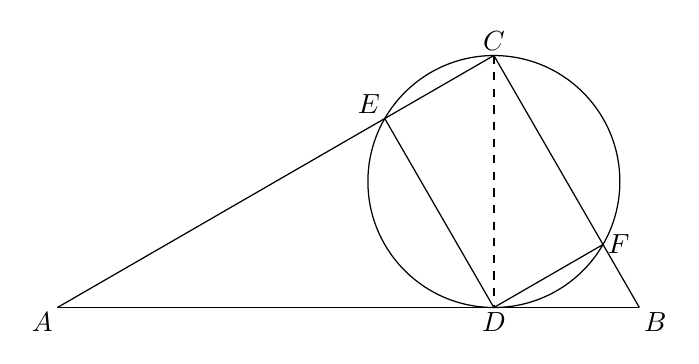
\begin{tikzpicture}[scale=1.6, line width=0.45pt,
  every node/.style={inner sep=1.5pt}]
  \coordinate (C) at (0,1);
  \coordinate (D) at (0,-1);
  \coordinate (E) at (-0.8660254,0.5);
  \coordinate (F) at (0.8660254,-0.5);
  \coordinate (A) at (-3.4641016,-1);
  \coordinate (B) at (1.1547005,-1);
  \draw (0,0) circle (1);
  \draw (A) -- (B);
  \draw (A) -- (C);
  \draw (C) -- (B);
  \draw (E) -- (D);
  \draw (D) -- (F);
  \draw[dashed] (C) -- (D);
  \node[anchor=south] at (C) {$C$};
  \node[anchor=south east] at (E) {$E$};
  \node[anchor=north] at (D) {$D$};
  \node[anchor=west] at (F) {$F$};
  \node[anchor=north east] at (A) {$A$};
  \node[anchor=north west] at (B) {$B$};
\end{tikzpicture}
\end{center}
\nopagebreak[4]
\end{question}
\begin{question}
\gkti{9}试问数列 $\lg100$，$\lg\left(100\sin\dfrac{\pi}{4}\right)$，$\lg\left(100\sin^2\dfrac{\pi}{4}\right)$，$\cdots$，$\lg\left(100\sin^{n-1}\dfrac{\pi}{4}\right)$ 前多少项的和的值最大？并求这最大值。（$\lg2=0.301$）

\end{question}
\begin{question}
\gkti{10}设等腰 $\triangle OAB$ 的顶角为 $2\theta$，高为 $h$。

（1） $\triangle OAB$ 内有一动点 $P$，到三边 $OA$、$OB$、$AB$ 的距离分别为 $|PD|$、$|PF|$、$|PE|$，并且满足关系 $|PD|\cdot|PF|=|PE|^2$。求 $P$ 点的轨迹；

（2） 在上述轨迹中定出点 $P$ 的坐标，使得 $|PD|+|PE|=|PF|$。

\end{question}